\documentclass[../notes.tex]{subfiles}
\graphicspath{{\subfix{../images/}}, {\subfix{../}}}

\begin{document}

\chapter{Superconductivity}

At the end of the 19th and the beginning of the 20th century, cooling technology made great progress.
Liquifying gases, were able to reach temperatures as low as \(\qty{4}{\kelvin}\) (the boiling point of Helium).
Using that, SC was discovered in mercury in 1911 by Heike Onnes \cite{onnesFurtherExperimentsLiquid1991}.
Superconductivity describes the phenomenon of the electrical resistance of a material suddenly dropping to zero below a critical temperature \(T_C\).
Discovery of Meissner effect, perfect expulsion of external magnetic fields in 1933 \cite{meissnerNeuerEffektBei1933}.
This started almost half a century of intensive theoretical research, which culminated in John Bardeen, Leon Cooper and J. Robert Schrieffer developing the microscopic theory now know as BCS theory \cite{bardeenTheorySuperconductivity1957}.
1986 and 1987: discovery of superconductivity with very high \(T_C\) found in cuprates \cite{bednorzPossibleHighTc1986,uchidaHighTcSuperconductivity1987}.
Cuprate superconductors are made up of layers of cooper oxide and charge reservoirs in between.
The specific charge reservoir layers determine the properties of the SC and varying them lead to a rich zoo of materials with high \(T_C\)  \cite{rybickiPerspectivePhaseDiagram2016}.

Most current technical applications of superconductors rely on the fact that superconducting wires can carry much higher currents that ordinary wires and thus produce much larger magnetic fields.
The largest commercial application to date is in magnetic resonance imaging, a medical technique using strong magnetic fields and field gradients \cite{rinckMagneticResonanceMedicine}.
Technical applications in research are much wider, ranging from strong superconducting magnets in the LHC \cite{tollestrupDevelopmentSuperconductingMagnets2008} and other particle accelerators over detectors of single photons in astrophysics \cite{irwinTransitionEdgeSensors2005} to extremely sensitive measurement devices for magnetic fields \cite{koelleHightransitiontemperatureSuperconductingQuantum1999, faleyHighTcSQUIDBiomagnetometers2017}.

Since the first discovery of SC in cuprates, there has been a lot of work to develop superconductors with higher transition temperatures.
One interesting development in is in twisted multilayer systems, first realized as twisted bilayer Graphene \cite{caoUnconventionalSuperconductivityMagicangle2018}.
In comparison to the complex crystal structure of e.g. the Cuprates, twisted multilayer systems have a very simple structure and can be tuned very easily: the angle of twist between the layers can be easily accessed experimentally.
The defining feature of these systems are flat electronic bands due to folding of the Brilluoin zone.
Superconductivity in these systems is enhanced due to the fact that in the flat bands, interactions between the electrons are very strongly enhanced.
Thus these systems are a very interesting playground to study strongly correlation effects in general and superconductivity in particular.

This chapter: introduction to the mean-field BCS theory in \cref{sec:bcs-theory}, GL-theory in \cref{sec:Ginzburg-Landau theory of superconductivity} and


\section{Ginzburg-Landau theory of superconductivity}\label{sec:Ginzburg-Landau theory of superconductivity}

Following~\cite[ch. 11]{colemanIntroductionManyBodyPhysics2015}.

\subsection{Order parameter concept}

Landau theory: phase transitions (e.g.\ iron becomes magnetic, water freezes, superfluidity/superconductivity) are associated with the development of an order parameter when the temperature drops below the transition temperature \(T_C\).
\begin{equation}
	\vert \psi \vert =
	\begin{cases}
		0\;,\; T > T_C \\
		\vert \psi_0 \vert > 0 \;,\; T < T_C
	\end{cases}
\end{equation}
Landau theory does not need microscopic expression for order parameter, it provides corse-grained description of the properties of matter.
The order parameter description is good at length scales above \(\xi_0\), the coherence length (e.g.\ size of Cooper pairs for SC).
On length scales above \(\xi_0\), the order parameter behaves as a smoothly varying function.

\subsection{Ginzburg-Landau theory}

\paragraph{Landau theory}

Basic idea of Landau theory: write free energy as function \(F[\psi]\) of the order parameter.
Region of small \(\psi\), expand free energy of many-body system as simple polynomial:
\begin{equation}
	f_{L} = \frac{1}{V} F[\psi] = \frac{r}{2} \psi^2 + \frac{u}{4} \psi^4
\end{equation}
Provided \(r\) and \(u\) are greater that \(0\): minimum of \(f_L [\psi])\) lies at \(\psi = 0\).
Landau theory assumes: at phase transition temperature \(r\) changes sign, so:
\begin{equation}
	r = a(T - T_C)
\end{equation}
Minimum of free energy occurs for:
\begin{equation}
	\psi = \begin{cases}
		0 \\
		\pm \sqrt{\frac{a (T_C - T)}{u} }
	\end{cases}
\end{equation}

Two minima for free energy function for \(T < T_C\).
With this, we can extract \(T_C\) from the knowledge of the dependence of \(\vert \psi \vert^2\) on \(T\) via a linear fit.
This is only valid for an area near \(T_C\) (where Landau theory holds), but can be used to get \(T_C\) from microscopic theories.

Going from a one to a \(n\)-component order parameters, OP acquires directions and magnitude.
Particularly important example: complex or two component order parameter in superfluids and superconductors:
\begin{equation}
	\psi = \psi_1 + \iu \psi_2 = \vert \psi \vert e^{\iu \phi}
\end{equation}
The Landau free energy takes the form:
\begin{equation}
	f[\psi] = r(\psi^* \psi) + \frac{u}{2} (\psi^* \psi)^2
\end{equation}
As before:
\begin{equation}
	r = a(T - T_C)
\end{equation}

Figure~\ref{fig:Landau free energy mexican hat potential} shows the Landau free energy as function of \(\psi\).

\begin{figure}[t]
	\centering
	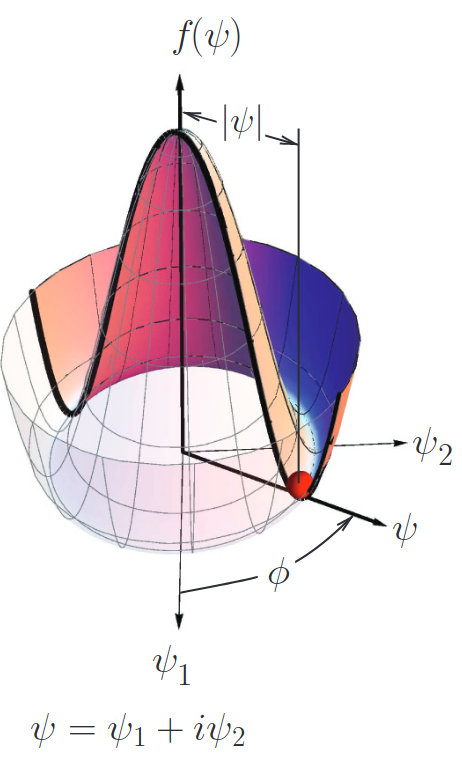
\includegraphics[width=0.3\textwidth]{images/landau free energy mexican hat}
	\caption{Mexican hat potential}
	\label{fig:Landau free energy mexican hat potential}
\end{figure}

Rotational symmetry, because free energy is independent of the global phase of the OP:
\begin{equation}
	f [\psi] = f [e^{\iu a } \psi]
\end{equation}
In this `Mexican hat' potential: order parameter can be rotated continuously from one broken-symmetry state to another.
If we want the phase to be rigid, we need to introduce an
There is a topological argument for the fact that the phase is rigid.
This leads to Ginzburg-Landau theory.
Will see later: well-defined phase is associated with persistent currents or superflow.

\paragraph{Ginzburg-Landau theory}

Landau theory: energy cost of a uniform order parameter, more general theory needs to account for inhomogenous order parameters, in which the amplitude varies or direction of order parameter is twisted -> GL theory.
First: one-component, `Ising' order parameter.
GL introduces additional energy \(\delta f \propto \vert \Delta \psi \vert^2\), \(f_{GL} [\psi, \Delta \psi] = \frac{s}{2} \vert \Delta \psi \vert^2 + f_L [\psi(s)]\), or in full:
\begin{equation}
	f_{GL} [\psi, \Delta \psi, h] = \frac{s}{2} (\Delta \psi)^2 + \frac{r}{2} \psi^2 + \frac{u}{4} \psi^4
\end{equation}
GL theory is only valid near critical point, where OP is small enough to permit leading-order expansion.
Dimensional analysis shows: \(\frac{s}{r} = L^2\) has dimension of length squared.
Length scale introduced by the gradient term: correlation length
\begin{equation}
	\xi (T) = \sqrt{\frac{s}{\vert r(T) \vert}} = \xi_0 \left\vert 1 - \frac{T}{T_C} \right\vert^{-\frac{1}{2}}
\end{equation}
sets characteristic length scale of order-parameter fluctuations, where
\begin{equation}
	\xi_0 = \xi (T = 0) = \sqrt{\frac{s}{\alpha T_C}}
\end{equation}
is a measure of the microscopic coherence length.
Near transition \(\xi (T)\) diverges, but far from transition it becomes comparable with the coherence length.

\paragraph{Complex order and superflow}

Now: GL theory of complex or two-component order parameters, so superfluids and superconductors.
Heart of discussion: emergence of a `macroscopic wavefunction', where the microscopic field operators \(\hat{\psi}(x)\) acquire an expectation value:
\begin{equation}
	\braket{\hat{\psi} (x)} = \psi (x) = \vert \psi (x) \vert e^{\iu \theta(x)}
\end{equation}
Reminder: Field operators are the real space representations of creation/annihilation operators.
They can be thought of the super position of all ways of creating a particle at position \(x\) via the basis coefficients.

Magnitude determines density of particles in the superfluid:
\begin{equation}
	\vert \psi(x) \vert^2 = n_s (x)
\end{equation}
Density operator is
\begin{equation}
	\hat{\rho} = \hat{\psi} (x) \hat{\psi^{\dagger}} (x)
\end{equation}
so expectation value of that is the formula above.

Twist/gradient of phase determines superfluid velocity:
\begin{equation}
	\vb{v}_s (x) = \frac{\hbar}{m} \Delta \phi (x)
\end{equation}
We will derive this later in the chapter.
Counterintuitive from quantum mechanics: GL suggested that \(\Phi(x)\) is a macroscopic manifestation of a macroscopic number of particles condensed into precisely the same quantum state.
Emergent phenomenon, collective properties of mater not a-priori self-evident from microscopic physics.

GL free energy density for superfluid (with one added term in comparison to Landau energy):
\begin{equation}
	f_{GL} [\psi, \Delta \psi] = \frac{\hbar^2}{2m} \vert \Delta \psi \vert^2 + r \vert \psi \vert^2 + \frac{u}{2} \vert \psi \vert^4
\end{equation}
Interpreted as energy density of a condensate of bosons in which the field operator behaves as a complex order parameter.
\todo{energy density of bosonic field? -> for comparison!}
Gives interpretation of gradient term as kinetic energy:
\begin{equation}
	s \vert \Delta \psi \vert^2 = \frac{\hbar^2}{2m} \braket{\Delta \hat{\psi}^{\dagger} \Delta \hat{\psi}} \implies s = \frac{\hbar^2}{2m}
\end{equation}
As in Ising order: correlation length/GL-coherence length governs characteristic range of amplitude fluctuations of the order parameter:
\begin{equation}
	\xi = \sqrt{\frac{s}{\vert r \vert}} = \sqrt{\frac{\hbar^2}{2m \vert r \vert}} = \xi_0 (1 - \frac{T}{T_C})^{-\frac{1}{2}}
\end{equation}
\todo{Compare with Ising order, especially dependence on \(T\)}
where \(\xi_0 = \xi(T=0) = \sqrt{\frac{\hbar^2}{2 m a T_C}}\) is the coherence length.
Beyond this length: only phase fluctuations survive.
\todo{Compare with Ising order. Is that derived or postulated?}
Freeze out fluctuations in amplitude (no \(x\)-dependence in amplitude) \(\psi(x) = \sqrt{n_s} e^{\iu \phi(x)}\), then \(\Delta \psi = \iu \Delta \phi \psi\) and \(\vert \Delta \psi \vert^2 = n_s (\Delta \phi)^2\), dependency of kinetic energy on the phase twist is (bringing it into the form \(\frac{m}{2} v^2\)):
\begin{equation}
	\frac{\hbar^2 n_s}{2m} (\Delta \phi)^2 = \frac{m n_s}{2} (\frac{\hbar}{m} \Delta \phi)^2
\end{equation}
So twist of phase results in increase in kinetic energy, associated with a superfluid velocity:
\begin{equation}
	\vb{v}_s = \frac{\hbar}{m} \Delta \phi
\end{equation}

For interpretation of superfluid states: coherent states.
These are eigenstates of the field operator
\begin{equation}
	\hat{\psi}(x) \ket{\psi} = \psi (x) \ket{\psi} 
\end{equation}
and don't have a definite particle number.
Importantly, this small uncertainty in particle number enables a high degree of precision in phase (which is the property of a condensate).

Phase rigidity and superflow: in GL theory, energy is sensitive to a twist of the phase.
Substitute \(\psi = \vert \psi \vert e^{\iu \phi}\) into GL free energy, gradient term is:
\begin{equation}
	\Delta \psi = (\Delta \vert \psi \vert + \iu \Delta \phi \vert \psi \vert) e^{\iu \phi}
\end{equation}
So:
\begin{equation}
	f_{GL}  = \frac{\hbar}{2m} \vert \psi \vert^2 (\Delta \phi)^2 + \left[ \frac{\hbar}{2m} (\Delta \vert \psi \vert)^2 + r \vert \psi \vert^2 + \frac{u}{2} \vert \psi \vert^4 \right]
\end{equation}
The second term resembles GL functional for an Ising order parameter, describes energy cost of variations in the magnitude of the order parameter.

\todo{Here: particle-current operator, especially for coherent state, connection with phase twist}


\section{Superconducting length scales from the constraint of finite-momentum pairing}

From~\cite{wittBypassingLatticeBCSBEC2024}.

In most materials: Cooper pairs do not carry finite center-of-mass momentum.
In presence of e.g.\ external fields or magnetism: SC states with FMP might arise.

Theory/procedure in the paper: enforce FMP states via constraints on pair-center-of-mass momentum \(\vb{q}\), access characteristic lenght scales \(\xi_0, \lambda_L\) through analysis of the momentum and temperature-dependent OP\@.
Constrain for FF-type pairing:
\begin{equation}
	\psi_{\vb{q}} (\vb{r}) = \vert \psi_{\vb{q}} \vert e^{\iu \vb{q} \vb{r}}
\end{equation}

\todo{Finish up the discussion of Niklas paper}

\section{Mean-field theory of superconductivity}\label{sec:bcs-theory}

\subsection{BCS theory}

Following \cite[ch. 14]{colemanIntroductionManyBodyPhysics2015}.

Theoretical description of SC: 1957 by John Bardeen, his postdoc Leon Cooper and the graduate in the group, J. Robert Schrieffer \cite{bardeenTheorySuperconductivity1957}.
Description is based on the fact, that the Fermi sea is unstable towards development of bound pairs under arbitrarily small attraction \cite{cooperBoundElectronPairs1956}.
These bound electrons show bosonic behaviour and 
\todo{Why supercurrent in BCS theory?}

\todo{BCS hamiltonian, pairing}
This model Hamiltonian

The final element in this description was the origin of the attractive interaction between electrons, which Bardeen, Cooper and Schrieffer identified as a retarded electron-phonon interaction \cite{bardeenTheorySuperconductivity1957}.
This so-called BCS-theory of superconductivity is very successful in explaining experimental results in many compounds, 
Surprisingly, it
\todo{What is explained by phononic pairing}

\todo{Other pairing interactions can be taken, gives explanations for a lot of different SCs}

%BCS-theory gave a microscopic explanation to a phenomenological description of superconductivity pioneered by Fritz London in 1937 \cite{londonNewConceptionSupraconductivity1937}.
%This descriptions is based on a one-particle wave function \(\phi (x)\)

%Later, this one-particle wavefunction was identified as the order parameter in the developing GL-theory of phase transitions \cite{landauTheorySuperconductivity1965}.
%GL-theory is discussed in more detail in \cref{sec:Ginzburg-Landau theory of superconductivity}.
%This explains the Meissner effect and in turn the supercurrent.

\subsection{Mean field-theory on the attractive Hubbard model}

Hubbard model is the simplest model for interactions

\cite{qinHubbardModelComputational2022}

\todo{Some relevance of the repulsive Hubbard model}

\todo{Motivation for taking a negative U}

\cite{micnasSuperconductivityNarrowbandSystems1990}

\todo{Phase diagram }

\paragraph{Multi-band BCS theory on the Hubbard model}

Fourier transformation:
\begin{equation}
	H_{int} = - \frac{1}{N^2} \sum_{\alpha, \vb{k}_{1, 2, 3, 4}} U_{\alpha} e^{\iu (\vb{k}_1 + \vb{k}_4 - \vb{k}_1 - \vb{k}_3) r_{i \alpha}}  c_{\vb{k}_1 \alpha \uparrow}^{\dagger} c_{\vb{k}_3 \alpha \downarrow}^{\dagger} c_{\vb{k}_2 \alpha \downarrow} c_{\vb{k}_4 \alpha \uparrow}
\end{equation}
Impose zero-momentum pairing: \(\vb{k}_1 + \vb{k}_3 = 0\) and \(\vb{k}_2 + \vb{k}_4 = 0\):
\begin{align}
	H_{int} = - \sum_{\alpha, \vb{k}, \vb{k}^{\prime}} U_{\alpha} c_{\vb{k} \alpha \uparrow}^{\dagger} c_{-\vb{k} \alpha \downarrow}^{\dagger} c_{-\vb{k}^{\prime} \alpha \downarrow} c_{\vb{k}^{\prime} \alpha \uparrow}
\end{align}
Mean-field approximation:
\begin{align}
	H_{int} \approx \sum_{\alpha, \vb{k}} (\Delta_{\alpha} c_{\vb{k} \alpha \uparrow}^{\dagger} c_{-\vb{k} \alpha \downarrow}^{\dagger} + \Delta_{\alpha}^* c_{-\vb{k} \alpha \downarrow} c_{\vb{k} \alpha \uparrow})
\end{align}
with
\begin{align}
	\Delta_{\alpha} &= - U_{\alpha} \sum_{\vb{k}^{\prime}} \braket{c_{-\vb{k}^{\prime} \alpha \downarrow} c_{\vb{k}^{\prime} \alpha \uparrow}} \\
	\Delta_{\alpha}^* &= - U_{\alpha} \sum_{\vb{k}^{\prime}} \braket{c_{\vb{k}^{\prime} \alpha \uparrow}^{\dagger} c_{-\vb{k}^{\prime} \alpha \downarrow}^{\dagger}}
\end{align}
This gives the BCS mean field Hamiltonian:
\begin{align}
	H_{BCS} = \sum_{\vb{k} \alpha \beta \sigma} [H_{0, \sigma} (\vb{k})]_{\alpha \beta} c_{\vb{k} \alpha \sigma}^{\dagger} c_{\vb{k} \beta \sigma}
	-\mu \sum_{\vb{k} \alpha \sigma} n_{\vb{k} \alpha \sigma}
	+ \sum_{\alpha, \vb{k}} (\Delta_{\alpha} c_{\vb{k} \alpha \uparrow}^{\dagger} c_{-\vb{k} \alpha \downarrow}^{\dagger} + \Delta_{\alpha}^* c_{-\vb{k} \alpha \downarrow} c_{\vb{k} \alpha \uparrow})
\end{align}
with Nambu spinor
\begin{equation}
	\Psi_{\vb{k}} =
	\begin{pmatrix}
		c_{1, \vb{k} \uparrow} \\
		c_{2, \vb{k} \uparrow} \\
		c_{3, \vb{k} \uparrow} \\
		c_{1, -\vb{k} \downarrow}^{\dagger} \\
		c_{2, -\vb{k} \downarrow}^{\dagger} \\
		c_{3, -\vb{k} \downarrow}^{\dagger} \\
	\end{pmatrix}
\end{equation}
we have:
\begin{equation}
	H_{MF} = \sum_{\vb{k}} \Psi_{\vb{k}}^{\dagger} \mathcal{H} (\vb{k}) \Psi_{\vb{k}}
\end{equation}
with
\begin{equation}
	\mathcal{H} (\vb{k}) =
	\begin{pmatrix}
		H_{0, \uparrow} (\vb{k}) - \mu & \Delta \\
		\Delta^{\dagger} & - H_{0, \downarrow}^* (-\vb{k}) + \mu
	\end{pmatrix}
\end{equation}
with \(H_{0, \sigma}\) being the F.T. of the kinetic term and \(\Delta = diag(\Delta_1, \Delta_2, \Delta_3)\).

\todo{General multi-band mean field theory theory}

\paragraph{Self-consistent solution}

\todo{How to solve mean field theory self-consistently}

\paragraph{Finite momentum}

\todo{How to include finite momentum}

\end{document}
